\documentclass[11pt, a4paper]{article}
\usepackage[utf8]{inputenc}

\usepackage[margin=1in]{geometry} 
\usepackage{amsmath,amsthm,amssymb}
\usepackage[margin=1in]{geometry} 
\usepackage{amsmath,amsthm,amssymb}

\usepackage[slovene]{babel}
\usepackage{color}
\usepackage{graphicx}
\usepackage{amssymb}
\usepackage{amsmath}
\usepackage{mathtools}
\usepackage{commath}
\usepackage{ragged2e}
\usepackage[T1]{fontenc}
\usepackage[normalem]{ulem}
\usepackage{amsthm}
\usepackage{esvect}
\usepackage{float}
\usepackage{calrsfs}
\DeclareMathAlphabet{\pazocal}{OMS}{zplm}{m}{n}
\newcommand{\Ga}{\mathcal{G}}
\mathtoolsset{showonlyrefs} 

\newcommand\setItemnumber[1]{\setcounter{enumi}{\numexpr#1-1\relax}}


\newtheorem{theorem}{Trditev}[section]
\newtheorem{corollary}{Posledica}[section]
\newtheorem{lemma}[section]{Lema}
\theoremstyle{definition}
\newtheorem{definition}{Definicija}[section]
\theoremstyle{example}
\newtheorem{example}[section]{Primer}
\theoremstyle{izrek}
\newtheorem{izrek}[section]{Izrek}

\begin{document}
\begin{center}
\thispagestyle{empty}
\parskip=14pt%
\vspace*{3\parskip}%
\begin{Huge} Uporaba ultrazvoka \end{Huge}

By

Matic Tonin

ID No. (28181098)

Mentor 

(Rok Dolenec)

\rule{7cm}{0.4pt}

Pod okvirom:

FAKULTETE ZA FIZIKO IN MATEMATIKO, LJUBLJANA

22. 3. 2020

\end{center}
\pagebreak
\section{Naloga}
\begin{enumerate}
\item Opazuj odboj longitudinalnega ultrazvocnega valovanja na razlicnih ploskvah priloženega
merjenca nepravilnih oblik z izvrtinami in zarezami. Kalibriraj skalo na
zaslonu osciloskopa v mm poti valovanja v jeklu.
\item Poišci odboj na izvrtini premera 1mm in doloci njen položaj glede na zunanje
ploskve merjenca. Oceni globinsko ostrino meritve.
\item Doloci hitrost longitudinalnega in transverzalnega ultrazvocnega valovanja v jeklu
in aluminiju, ali v drugem materialu. Uporabi ultrazvocni interferometer. Izracunaj
prožnostni modul E, strižni modul G in Poissonovo število $\mu$.
\end{enumerate}

\section{Meritve}
\subsection{Kalibracija skale na zaslonu}
Za ta del naloge smo najprej izračunali, glede na potovanje našega signala po snovi, kolikšna je njegova hitrost. 
Izmerili smo, 
\begin{table}[ht]
	\centering
	\begin{tabular}{|c|c|c|}
		\hline
		Smer & d [mm] & t[$\mu$s]  \\
		\hline
		\hline
		x-smer& 91 & 31.2\\
		\hline
		y-smer& 100 & 34.8 \\
		\hline
		z-smer& 24.5 & 9.2\\
		\hline
		\end{tabular}
		\caption{Prikaz kalibracije hitrosti glede na izbiro površine}
		\label{tab:FirstTable}
\end{table}

S to tabelo lahko izračunamo nato hitrost za naš predmet, ker vemo da je $c=\frac{2d}{t}$:

\begin{figure}[htp]
    \centering
    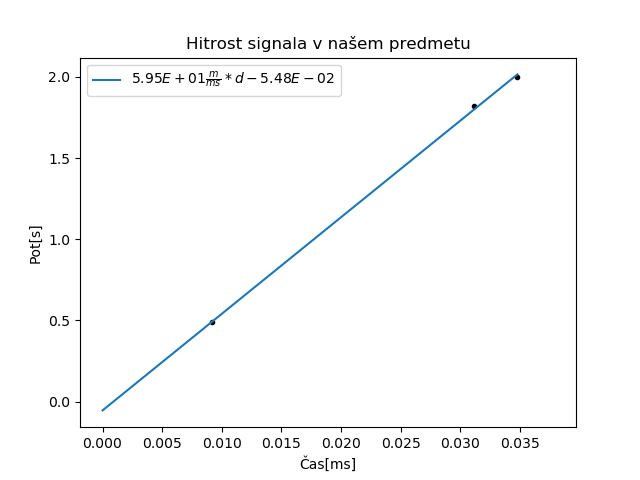
\includegraphics[width=10cm]{Hitrost.png}
    \caption{Graf odvisnosti poti od časa potovanja po snovi}
\end{figure}
Torej je hitrost potovanja signala po snovi enaka:
$$\underline{\underline{c=5950 \frac{m}{s} +/- 447 \frac{m}{s}}}$$

\pagebreak
\textbf{Napaka meritve hitrosti}
Ocena naše napake je:
\begin{enumerate}
\item Ocena napake meritve debeline:\\
Ker smo merili z milimeterskim merilom je napaka potem kar 0.5 mm. 
\item Ocena napake meritve časa: \\
Ker smo odčitavali iz osciloskopa in si lahko pomagali s funkcijo Cursor, ki nam pomaga določiti točno lokacijo novega signala, ocenjujem napako 0.5 $mu$s. 
\end{enumerate}

\subsection{Odboj pri izvrtini}
Da smo izmerili lokacijo izvrtine, smo signalno sondo postavili najprej na nekaj mm pred izrvtino ter na določenih lokacijah merili, kako se spreminja čas odboja z premikanjem naše sonde.
Izmerili smo, \begin{table}[ht]
	\centering
	\begin{tabular}{|c|c|c|c|}
		\hline
		Smer & t[$\mu$s] &  $d [mm]=\frac{ct}{2}$ & dejanske vrednosti\\
		\hline
		\hline
		1 & 31.6 & 94 & 91\\
		\hline
		2 & 29.4 & 101 & 100\\
		\hline
		3 & 34.8 & 85 & 84\\
		\hline
		\end{tabular}
		\caption{Meritve lokacije luknje v našem predmetu}
		\label{tab:FirstTable}
\end{table}

Vidimo, da se naše vrednosti zelo ujemajo z vrednostmi, ki smo jih dejansko izmerili z merilom. 
\begin{figure}[htp]
    \centering
    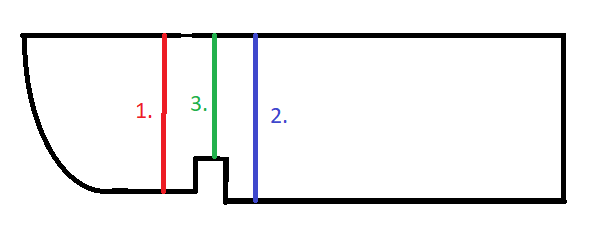
\includegraphics[width=10cm]{Slika luknje.png}
    \caption{Grafični prikaz meritev iz tabele 2. }
\end{figure}

Za globinsko ostrino slike smo nastavili merilnik kot je bilo prikazano na Sliki 3. ter nato opazovali, kako se izoblikujejo odboji na osciloskopu. 

\begin{figure}[htp]
    \centering
    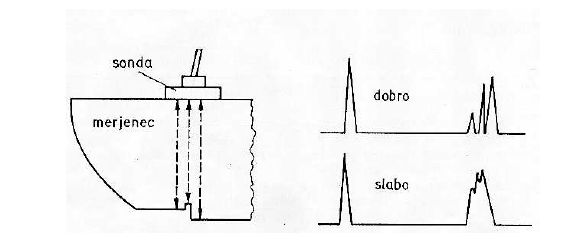
\includegraphics[width=10cm]{Globinska ostrina.png}
    \caption{Prikaz opazovanja globinske ostrine }
\end{figure}

Na mojih meritvah sem ocenil, da je bila debelina reže v enotah signala vredna okoli $3 \mu s$. Iz tega lahko izračunamo, da je globina naše jame $d_{jame}=1$ mm. \\
Signal se je pojavil pri 28.5 $\mu $s, kar pomeni, da je globinska ostrina naše sonde: 
$$d_{ostrina}= 0.085 m $$

\subsection{Hitrost longituginalnega in transferzalnega valovanja}

Kot prvo smo morali izmeriti temperaturo zraka, da smo tako lahko določili, kolikšna je hitrost valovanja v vodi. 
Torej, če sta $k=2.5 \frac{m}{Ks}$, $T_0=20$ stopinj in $c_0=1483.1 \frac{m}{s}$: \\
\begin{table}[ht]
	\centering
	\begin{tabular}{|c|c|c|c|}
		\hline
		Temperatura & $c=c_0+k(T-T_0) \frac{m}{s}$ &  Napaka T & Rezultat z napako\\
		\hline
		\hline
	  	22.5 stopinj & 1489.35  & 0.1 stopinje => $\delta T=0.0044 $ & 1489.35 +/- 6.617 $\frac{m}{s}$ \\
		\hline
		\end{tabular}
		\caption{Meritve hitrosti zvoka v vodi}
		\label{tab:FirstTable}
\end{table}

Da pa bi izmerili hitrosti valovanja v vodi in v izbranem merjencu pa lahko zapišemo tako.
Če z premikanjem ploščice odboja preverjamo, kje se časa odboja v vodi in v snovi ujemata, lahko dobimo enačbo, ki je: 
\begin{center}
$t_{v}=\frac{2d_{v}}{c_v}$ \quad
\medskip
$t_{m}=\frac{2nd_{m} }{c_m}$ \\
\medskip
$t_{v}=t_{m} $ \\
\medskip
$c_{m}= c_{v} d_{m} \frac{n}{d_{v}}$
\end{center}
Ker smo opravili več meritev lahko zapišemo razmerje razdalje z številom odbojev kot nek koeficient premice, ki ga uprizorimo na grafu. Torej: 
$$ K= \frac{d_v}{n}$$
Izmerimo lahko brez težav debeline naših predmetov in sicer: 
\begin{table}[ht]
	\centering
	\begin{tabular}{|c|c|}
	\hline 
	Snov & debelina z napako \\
	\hline 
	\hline 
	Jeklo &$2,51 \pm 0,01 \text{cm}$\\
	\hline 
	Aluminij &$2,62 \pm 0,01 \text{cm} $\\
	\hline 
	Medenina& $2,52 \pm 0,01\text{cm}$\\
	\hline 
		\end{tabular}
		\caption{Meritve debeline merjencev}
		\label{tab:FirstTable}
\end{table}
Tako lahko merimo hitrost transverzalnega in longituginalnega valovanja.
\subsubsection{Longitudinalnega valovanje}
Za merjenje longitudinalnega smo gledali, kdaj se pojavi ojačitev na naši sondi in sicer
\begin{table}[ht]
	\centering
	\begin{tabular}{|c|c|c|c|c|c|}
	\hline 
	Jeklo [n] & $d_v$ [cm] & Medenina [n] & $d_v$ [cm]& Aluminij [n] & $d_v$ [cm] \\ [1ex] 
	\hline 
	\hline 
	1 &	0.3 & 1 &  0.5 &1& 0.2\\
	\hline 
	2 & 0.9 & 2 & 1.3 &2& 0.8\\
	\hline 
	3 & 1.5 & 3 & 2.1 &3& 1.4\\
	\hline 
	4 & 2.1 & 4& 2.9 &4& 2.0\\
	\hline
		\end{tabular}
		\caption{Meritve razdalj odbojev}
		\label{tab:FirstTable}
\end{table}
Iz tega smo lahko lahko izmerili koeficiente $ K= \frac{d_v}{n}$ in nato izračunali hitrost valovanja v longitudinalni smeri $c_{m}= c_{v} d_{m} K^{-1}$.

\begin{table}[ht]
	\centering
	\begin{tabular}{|c|c|c|c|}
	\hline 
	Snov & Koeficient z napako & $c_{long}$ $[\frac{m}{s}]$ & Koeficient E [N/mm]\\ [1ex] 
	\hline 
	\hline 
	 Medenina & 7.00 $10^{-03}$ m& 4937 & 11000  \\ [0.5ex] 
	\hline 
	Aluminij & 5.9 & 6362 & 71000 \\[0.5ex] 
	\hline 
	Jeklo& 6.00  $10^{-03}$ & 6231 & 218500 \\[0.5ex] 
	\hline 
		\end{tabular}
		\caption{Meritve koeficientov in ocene hitrosti valovanja ter koeficienta E za longitudinalno valovanje}
		\label{tab:FirstTable}
\end{table}

Kako smo dobili koeficient E? \\

Če pogledamo enačbo:

$$c_{long}=\frac{E}{\rho}$$

vidimo, da imamo za izračun prožnostnega modula že vse podatke, če seveda imamo izračunan c, podane in tako lahko samo vstavimo v naš program, ki računa naklone premic. \\
\medskip

Dodajam pa še grafe za izračun koeficienta K za vse snovi. 
\begin{figure}[htp]
    \centering
    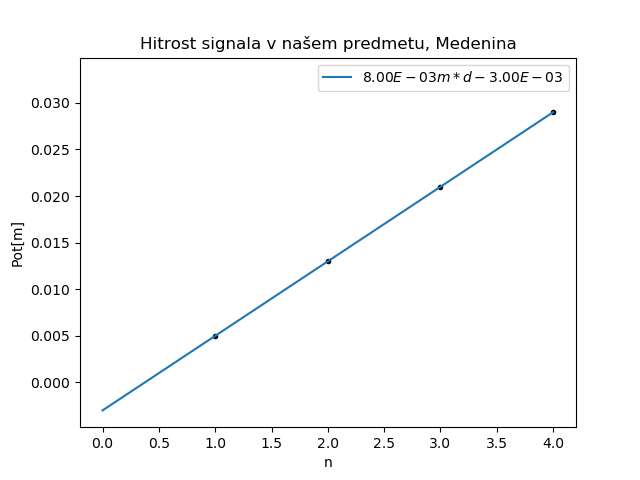
\includegraphics[width=10cm]{Medenina.png}
    \caption{Prikaz grafa odbojev v odvisnosti od poti v vodi, Medenina}
\end{figure}
\begin{figure}[htp]
    \centering
    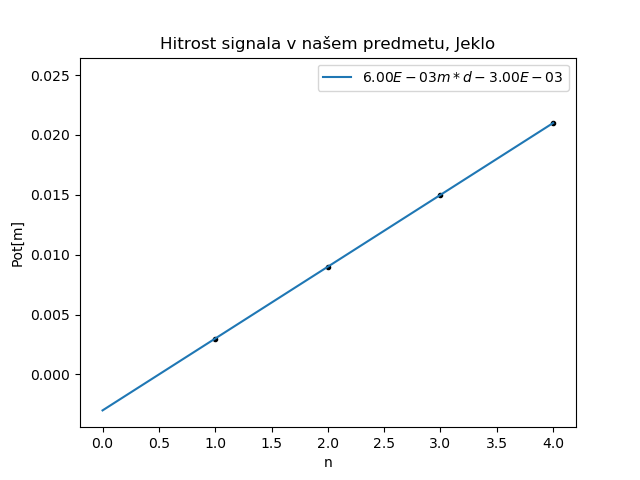
\includegraphics[width=10cm]{Jeklo.png}
    \caption{Prikaz grafa odbojev v odvisnosti od poti v vodi, Jeklo}
\end{figure}
\begin{figure}[htp]
    \centering
    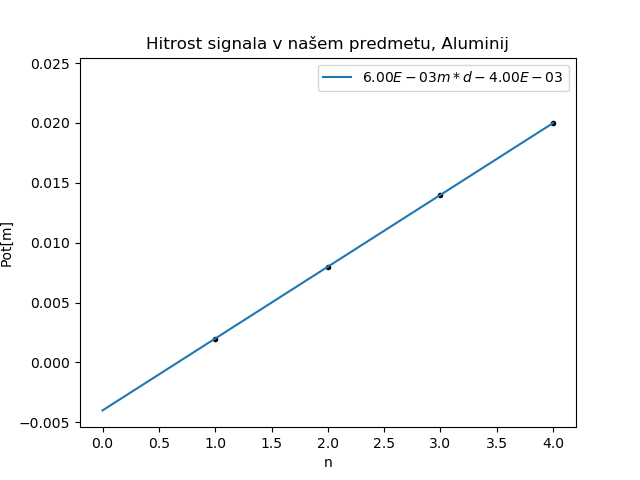
\includegraphics[width=10cm]{Aluminij.png}
    \caption{Prikaz grafa odbojev v odvisnosti od poti v vodi, Aluminij}
\end{figure}



\pagebreak
\textbf{DRUGI DEL VAJE,
\\ POJASNILO ZAKAJ GA NI IN KAKO BI SE MORAL IZVESTI:} \\

\medskip
Kot sem vam že v mailu navedel, na žalost 2 dela vaje nisem opravljal, saj je bil kabel za priključek Atenuatorja pokvarjen in so bile tako meritve neuporabne. 
Če pa bi dobil meritve, pa bi z njimi moral ravnati, tako kot za prvi del 3 naloge. Torej bi rabili izračunati hitrost valovaja po vsaki snovi in nato bi lahko določili, kakšno je Poissonovo število iz enačbe:

$$\mu=\frac{c_{long}^2-2c_{trans}^2}{2(c_{long}^2-c_{trans}^2)}$$

Kar je v resnici zgolj ta enačba z vstavljenim $c_{long}=\frac{E}{\rho}$.

$$c_{\text {trans }}^{2}=\frac{E}{2 \rho(1+\mu)}$$

Ko dobimo Poissonovo število za vsak material posebej, pa lahko dobimo tudi strižni modul ali G in sicer iz enačbe: 

$$\frac{G}{\rho}=c_{\text {trans }}^{2}=\frac{E}{2 \rho(1+\mu)}$$

Ampak ker meritve transverzalnega valovanja nisem uspel opraviti, sem lahko izračunal le Prožnostni modul za vsako snov, vse ostalo pa je na žalost odvisno od $c_{trans}$.



\end{document}